%%%%%%%%%%%%%%%%%%%%%%%%%%%%%%%%%%%%%%%%%
% Short Sectioned Assignment
% LaTeX Template
% Version 1.0 (5/5/12)
%
% This template has been downloaded from:
% http://www.LaTeXTemplates.com
%
% Original author:
% Frits Wenneker (http://www.howtotex.com)
%
% License:
% CC BY-NC-SA 3.0 (http://creativecommons.org/licenses/by-nc-sa/3.0/)
%
%%%%%%%%%%%%%%%%%%%%%%%%%%%%%%%%%%%%%%%%%

%----------------------------------------------------------------------------------------
%	PACKAGES AND OTHER DOCUMENT CONFIGURATIONS
%----------------------------------------------------------------------------------------

\documentclass[paper=letter, fontsize=11pt]{scrartcl} % A4 paper and 11pt font size

\usepackage[T1]{fontenc} % Use 8-bit encoding that has 256 glyphs
\usepackage{fourier} % Use the Adobe Utopia font for the document - comment this line to return to the LaTeX default
\usepackage[english]{babel} % English language/hyphenation
\usepackage{amsmath,amsfonts,amsthm} % Math packages

\usepackage[margin=1.0in]{geometry}
\usepackage{color}
\usepackage{graphicx}
\usepackage{caption}


\usepackage{sectsty} % Allows customizing section commands
\allsectionsfont{\centering \normalfont\scshape} % Make all sections centered, the default font and small caps

\usepackage{hyperref}
\usepackage{listings}
\lstset{ language=C++,
            keywordstyle=\color{red},
            basicstyle=\footnotesize,
            columns=fullflexible}
\usepackage{xcolor}
\usepackage{array}

%\numberwithin{equation}{section} % Number equations within sections (i.e. 1.1, 1.2, 2.1, 2.2 instead of 1, 2, 3, 4)
%\numberwithin{figure}{section} % Number figures within sections (i.e. 1.1, 1.2, 2.1, 2.2 instead of 1, 2, 3, 4)
%\numberwithin{table}{section} % Number tables within sections (i.e. 1.1, 1.2, 2.1, 2.2 instead of 1, 2, 3, 4)



%----------------------------------------------------------------------------------------
%	TITLE SECTION
%----------------------------------------------------------------------------------------

\newcommand{\horrule}[1]{\rule{\linewidth}{#1}} % Create horizontal rule command with 1 argument of height

\title{	
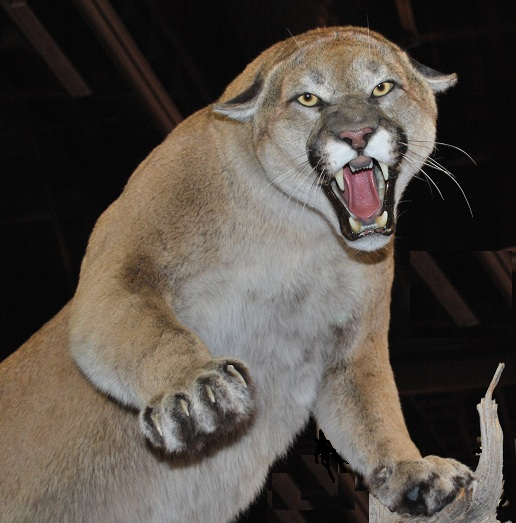
\includegraphics[width=3cm]{Cougar_Nevada}
\normalfont \normalsize 
%\textsc{APC 524} \\ [25pt] % Your university, school and/or department name(s)
\horrule{0.5pt} \\[0.4cm] % Thin top horizontal rule
\LARGE COUGAR (\textbf{CO}de \textbf{U}sually \textbf{G}enerates \textbf{A}xisymmetric \textbf{R}econstruction 1.0), \\ \Large An MHD Equilibrium Reconstruction Code: Final Report\\ % The assignment title
\horrule{2pt} \\[0.5cm] % Thick bottom horizontal rule
}

\author{Peter Bolgert (pbolgert@pppl.gov), Jonathan Ng (wng@pppl.gov), \\ Elizabeth Paul (epaul@princeton.edu), Jacob Schwartz (jschwart@pppl.gov)} % Your name

\date{\normalsize\today} % Today's date or a custom date

\begin{document}

\maketitle % Print the title

%----------------------------------------------------------------------------------------
%	Section 1
%----------------------------------------------------------------------------------------

\section{Project Objective / Summary}

Our goal was to write a program which solves the Grad-Shafranov equation (GSE) for axisymmetric plasmas in a user friendly manner.  The result is COUGAR, which stands for \textbf{CO}de \textbf{U}sually \textbf{G}enerates \textbf{A}xisymmetric \textbf{R}econstruction.  The main body of the code is written in C++, with a separate Python program for visualization.  The user can set code options either via the command line or text-based configuration file.  In the current version, some assumptions about the internal structure of the plasma must be made.  Future versions of the code will incorporate experimental measurements into the calculation.  For information on running COUGAR, see the README at \href{http://jonngwx.github.io/grad-shafranov/md__r_e_a_d_m_e.html}{\nolinkurl{jonngwx.github.io/grad-shafranov/md__r_e_a_d_m_e.html}}.

%----------------------------------------------------------------------------------------
%	Section 2
%----------------------------------------------------------------------------------------

\section{Theroetical Background}

\textbf{Notes}: The following material primarily follows Chapter 4 of \textit{Computational Methods in Plasma Physics}, by Stephen Jardin.  When there are discrepancies between that book and this document, the latter should be trusted as the former has misprints.  Also, SI units are used throughout.

\subsection{MHD equilibrium}

In magnetohydrodynamic (MHD) theory, a plasma equilibrium is described by the equation $\mathbf{\nabla} p = \mathbf{J} \times \mathbf{B}$, where $p$ is the scalar plasma pressure, $\mathbf{J}$ is the current density, $\mathbf{B} = \mathbf{\nabla} \times \mathbf{A}$ is the magnetic field, and $\mathbf{A}$ is the vector potential for the magnetic field.  We work in cylindrical coordinates $(R, \phi, z)$, and the plasma is assumed to be axisymmetric, i.e., $\partial / \partial \phi = 0$.

By introducing new functions $\Psi(R,z) \equiv -R A_{\phi}$ (called the flux function) and $g(R,z) \equiv R B_{\phi}$, we can rewrite the equilibrium equation in the following form, known as the Grad-Shafranov equation:
\begin{equation}
\Delta^{*} \Psi + \mu_0 R^2 \frac{dp}{d\Psi} + g \frac{dg}{d\Psi} = 0,
\end{equation}
where $\Delta^{*} \equiv R^2 \mathbf{\nabla} \cdot \frac{1}{R^2} \mathbf{\nabla}$ is called the toroidal elliptic operator. $p(\Psi)$ and $g(\Psi)$ are functions of $\Psi(R,z)$, the quantity that we are trying to solve for.  Thus $p(\Psi)$ and $g(\Psi)$ must be given (along with boundary conditions) for the problem to be fully specified.  Once the equation is solved, any other quantity of interest ($\mathbf{J}$, $\mathbf{B}$, etc.) can be calculated.  

\begin{figure}
\centering
\captionsetup{justification=centering,margin=3cm}
\caption[caption]{Cylindrical coordinates $(R,\phi,z)$.  Taken from "Computational Methods in Plasma Physics," Stephen Jardin.}

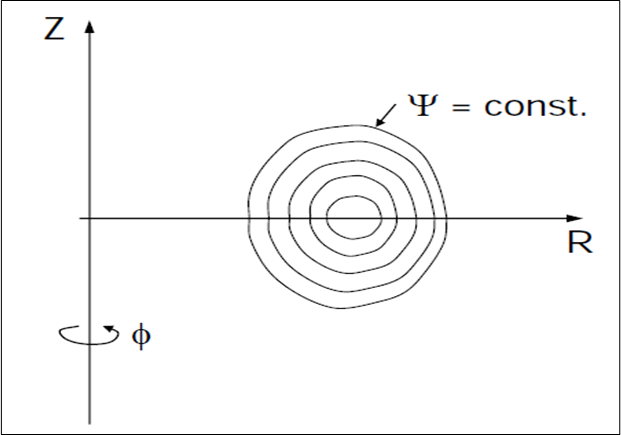
\includegraphics[width=0.35\textwidth]{coordinates}

\end{figure}

Without going into too much detail, it should be stated that the best MHD equilibria for confining plasmas are those which contain nested surfaces of constant $\Psi$ (known as flux surfaces), as in Figure 1.  It can be shown that a magnetic field line will always point tangentially to a given flux surface.  Since charged particles in the plasma follow field lines, the particles will stay on constant flux surfaces, resulting in good confinement. 



\subsection{Analytic Profiles vs Equilibrium Reconstruction}
As previously stated, the functions $p(\Psi)$ and $g(\Psi)$ must be supplied for a full specification of the problem.  In our code, we assumed simple analytic forms for these functions which roughly approximate real life experiments.  

Of course, in a real tokamak experiment, the functional forms of $g(\Psi)$ and $p(\Psi)$ are unknown.  Instead we must rely on a finite number of experimental measurements of $\Psi$ taken near the plasma boundary to deduce $p$ and $g$ as well as possible.  The approximate calculation of the flux function from these experimental measurements is known as Equilibrium Reconstruction, and will be implemented in a future version of COUGAR.  

\subsection{Algorithm when $p(\Psi)$ and $g(\Psi)$ are specified (current version of COUGAR)}



First rewrite the Grad-Shafranov equation as
\begin{equation}
\Delta^{*}\Psi = \mu_0 R J_{\phi} (R, \Psi),
\end{equation}
where $\mu_0 R J_{\phi} (R,\Psi) = - \big(\mu_0 R^2 \frac{d p}{d\Psi} + g \frac{d g}{d\Psi}\big)$, and $J_{\phi}$ is the current density in the $\phi$-direction.

Since the problem is non-linear (the right-hand-side of Eq.~(2) depends on $\Psi$), we use an iterative approach.  At each level of iteration, we solve a finite difference version of 
\begin{equation}
\Delta^{*}\Psi^{n} = \mu_0 R J_\phi (R, \Psi^{n-1}),
\end{equation}
where $n$ denotes the iteration level. The solution of $\Psi$ is plugged into the right-hand-side of Eq.~(3) for the next iteration.  This continues until the solution converges.  The linearized finite difference equation can be solved via a variety of methods. We currently have implemented two methods to solve Eq.~(3): the Gauss-Seidel method, and the method of Successive Over-Relaxation (SOR), which are explained in the next section.  

There is an additional nonlinearity relating to the boundary conditions.  Suppose that there are $N_c$ external coils outside of the computational boundary.  The flux function evaluated on the computational boundary $\Psi_b$ is then due to the plasma itself and the external coils:
\begin{equation}
\Psi^m_b (R',z') = \mu_0 \int_{plasma} G(R,z; R',z') J_{\phi} \mathop{dR} \mathop{dz} + \sum_{i=1}^{N_c} G(R_i^c,z_i^c; R',z') I_i,
\end{equation}





\begin{equation}
\Psi^m_b (R',Z') = \int_{b} \frac{dl}{R} G(R,Z; R',Z') \frac{\partial U^m}{\partial n} + \sum_{i=1}^{N_c} G(R_i^c,Z_i^c; R',Z') I_i,
\end{equation}
where $G$ is the Green's Function for the elliptic operator $\Delta^{*}$ (known analytically and stored in a look up table), $(R_i^c,Z_i^c)$ is the location of the $i$th coil with current $I_i$, and $U^m(R,Z)$ is a function which satisfies
\begin{align}
\Delta^{*} U^m &= \mu_0 R J_\phi (R, \Psi^{m-1}) \quad \mbox{inside the comp.~boundary} \\
U^m &= 0 \quad \mbox{on the boundary}.
\end{align}
The calculation of the boundary values using Eq.~4 is known as Von Hagenow's method (Lackner, Comp.~Phys. Comm.~12 (1976) 33-44).
The index $m$ in Eq.~(4) shows that the determination of the boundary condition is also an iterative process.  The $(m-1)$th value of $J_\phi$ is used to calculate $\Psi_b^m$.  

Given a set of boundary conditions, we can solve Eq.~(3) iteratively for $\Psi$.  This $\Psi$ is then used to calculate a new set of boundary conditions using Eq.~(4), and the process begins anew.  Ultimately, the process is a double-nested iteration which runs until the outer loop converges.  The process is depicted in Figure 2.

\begin{figure}
\centering
\captionsetup{justification=centering,margin=3cm}
\caption[caption]{Double-nested iteration loop. Taken from "Computational Methods in Plasma Physics," Stephen Jardin.}
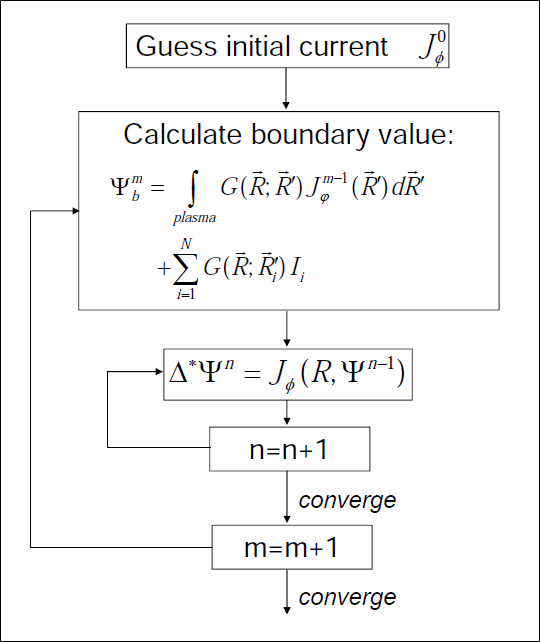
\includegraphics[width=0.45\textwidth]{algorithm}
\end{figure}

In summary, the \textbf{inputs} to the algorithm are an initial guess $J_\phi^0$ for the source function, the location of external coils $(R_i^c,Z_i^c)$ and their currents $I_i$, and the functional forms of $p(\Psi)$ and $g(\Psi)$.  The \textbf{output} is the value of $\Psi$ at each grid point in the $R-Z$ plane.  

\subsection{Algorithm using Experimental Measurements (for the future)}

In an experiment, $p(\Psi)$ and $g(\Psi)$ are unknown, but suppose we have $N_l$ measurements of the flux function $\Psi_l^{meas}$ near the plasma boundary (but within the computational boundary).  

First we expand our unknown functions in terms of basis functions (which our group must still determine):
\begin{equation}
p'(\Psi) = \sum_j \alpha_j y_j(\Psi), \quad gg'(\Psi) = \sum_j \beta_j y_j(\Psi).
\end{equation}
We can then write a formula for the computed value of $\Psi$ at the location $(R_l, Z_l)$ of each experimental measurement: 
\begin{equation}
\Psi_l^{comp}(R_l, Z_l) = \int_{plasma} G(R,Z; R_l,Z_l) J_\phi(R,\Psi,\alpha_j,\beta_j) dR dZ + \sum_{i=1}^{N_c} G(R_i^c,Z_i^c; R_l,Z_l) I_i.
\end{equation}
The computed values are compared to the measured values, and the minimization of an error function determines the values of $\alpha_j, \beta_j$ at that stage in the algorithm.   

Thus, the algorithm described in Section 1.4 is identical to that described in Section 1.3 (and depicted in Fig.~2), except that each time $\Psi$ is updated in the inner ($n$) loop, we also update the values of $\alpha_j, \beta_j$.  In summary, the \textbf{inputs} to the algorithm are an initial guess $J_\phi^0$ for the source function, the location of external coils $(R_i^c,Z_i^c)$ and their currents $I_i$, and the location of the experimental measurements $(R_l,Z_l)$ and their values $\Psi_l^{meas}$.  The \textbf{output} is the value of $\Psi$ at each grid point in the $R-Z$ plane.  



%----------------------------------------------------------------------------------------
%	Section 3
%----------------------------------------------------------------------------------------

\section{Code Organization / Class Structure}

The program is written in C++ with the visualization carried out separately using Python. The solver is called from the command line.  Options/parameters can be set on the command line or in a configuration file.  The location of external magnetic coils will also be contained in text files. Output will be written to text files or hdf5 files. 

The class structure of our code is explained below.  For more information, see the documentation website at \href{http://jonngwx.github.io/grad-shafranov/index.html}{\nolinkurl{jonngwx.github.io/grad-shafranov/index.html}}.
\\ \\

%%%%%%%%%%%%%%%% BIG CLASS TABLE%%%%%%%%%%%%%%%%%
\newgeometry{left=0.5cm, right=0.5cm, top=0.5cm, bottom=0.5cm}
\begin{table}
\small
\caption{Summary of COUGAR Classes}
\centering
\begin{tabular}{ | m{2.3cm} | p{8.9cm} | p{6cm}|}
    \hline Class Name & Methods (inherited methods only listed in parent class) & Brief Description \\
    \hline Grid & 
\begin{lstlisting}[belowskip=-\baselineskip, aboveskip=-0.5\baselineskip]
double celli(double r)
double cellj(double z) 
\end{lstlisting} 
   & Stores information about the computational grid. \\
   \hline Field & none & Container for 2d data and the grid \\ 
   \hline EllipticSolver & 
\begin{lstlisting}[belowskip=-\baselineskip, aboveskip=-0.5\baselineskip]
double norm_max (const Field &Psi, const Field &Psi_prev)
void iter(double omega)
void boundary (Field &Psi, const Field &Psi_prev) 
double norm()
virtual void step_1(const Field &jphi)=0
virtual void step(const Field &jphi)=0
virtual void coeff()=0
double residuals(const Field &Psi, const Field &Psi_prev) 
\end{lstlisting}
    & description of EllipticSolver \\ 
    \hline GaussSeidel &
\begin{lstlisting}[belowskip=-\baselineskip, aboveskip=-0.5\baselineskip]
void step_1(const Field &jphi)
void step(const Field &jphi)
void coeff()
\end{lstlisting} 
    & Implementation of EllipticSolver. Solves finite difference equation using Gauss-Seidel algorithm.\\
    \hline SOR & 
\begin{lstlisting}[belowskip=-\baselineskip, aboveskip=-0.5\baselineskip]
void step_1(const Field &jphi)
void step(const Field &jphi)
void coeff()
double omega()
\end{lstlisting}
    &Implementation of EllipticSolver.  Solves finite difference equation using Successive over-relaxation algorithm. \\ 
    \hline JSolver &
\begin{lstlisting}[belowskip=-\baselineskip, aboveskip=-0.5\baselineskip]
virtual void update(Field *jphi, Field *psi, Field *p, Field *g)=0
\end{lstlisting}
    & hello \\ 
    \hline JSolverAlpha &
\begin{lstlisting}[belowskip=-\baselineskip, aboveskip=-0.5\baselineskip]
void update(Field *jphi, Field *psi, Field *p, Field *g)
\end{lstlisting}
    & hello \\ 
    \hline JSolverNSTX & 
\begin{lstlisting}[belowskip=-\baselineskip, aboveskip=-0.5\baselineskip]
void update(Field *jphi, Field *psi, Field *p, Field *g)
\end{lstlisting}
    & ertertert \\ 
    \hline Boundary & 
\begin{lstlisting}[belowskip=-\baselineskip, aboveskip=-0.5\baselineskip]
virtual int CalcB(Field *jphi)
int LtoI(int l)
int LtoJ(int l)
double norm()
\end{lstlisting}
    & dffghfgh \\ 
    \hline SlowBoundary &
\begin{lstlisting}[belowskip=-\baselineskip, aboveskip=-0.5\baselineskip]
int CalcB(Field *jphi)
\end{lstlisting}
    & dfasdasd \\ 
    \hline Table &
\begin{lstlisting}[belowskip=-\baselineskip, aboveskip=-0.5\baselineskip]
virtual int load_from_tsv(const string filename, int header_lines=0)
int num_columns() const
int num_rows() const
double data(int row, int column) const
\end{lstlisting}
    & dfgdfgdfg \\ 
    \hline CoilData &
\begin{lstlisting}[belowskip=-\baselineskip, aboveskip=-0.5\baselineskip]
int load_from_tsv(const string filename, int header_lines=0) override
double r(int i) const
double z(int i) const
double current(int i) const
int num_coil_subregions() const
\end{lstlisting}
    & dfgdfgdfg \\ 
    \hline Critical &
\begin{lstlisting}[belowskip=-\baselineskip, aboveskip=-0.5\baselineskip]
void Psi_search(double r, double z, double *dr, double *dz)
void Psi_magnetic(double r, double z, double *rcrit, 
	double *zcrit, double *Psi_min)
double Psi_limiter ()
void update ()
bool find_saddle (double &r, double &z)
\end{lstlisting}
    & dfgdfgdg \\ 
    \hline Interpolate & 
\begin{lstlisting}[belowskip=-\baselineskip, aboveskip=-0.5\baselineskip]
double F (double r, double z) const
double F_r (double r, double z) const
double F_rr (double r, double z) const
double F_rz (double r, double z) const
double F_zz (double r, double z) const
double F_z (double r, double z) const
void updateInterpolation(double r, double z)
void PrintAmnCoefficients()
\end{lstlisting}
    & fsdfsdfsdf \\ 
    \hline GradOutput & 
\begin{lstlisting}[belowskip=-\baselineskip, aboveskip=-0.5\baselineskip]
virtual void write_output(const char *filename)=0
void parse_outputs(const char *outputs)
bool find(Output out)
\end{lstlisting}
    & dfgdfgd \\ 
   \hline GradOutputHdf & 
\begin{lstlisting}[belowskip=-\baselineskip, aboveskip=-0.5\baselineskip]
void write_output(const char *filename)
\end{lstlisting}
     & dfgfdfgdf \\ 
    \hline GradOutputTxt &
\begin{lstlisting}[belowskip=-\baselineskip, aboveskip=-0.5\baselineskip]
void write_output(const char *filename)
\end{lstlisting}
    & dfgdfgdf \\ 
    \hline
\end{tabular}
\end{table}
%%%%%%%%%%%%%%% END BIG CLASS TABLE %%%%%%%%%%%%%%%

\restoregeometry
The following C++ interfaces will be required and should be self-contained
\begin{itemize}
\item Elliptic solver - This is used to invert the elliptic operator $\Delta^*$ and solve for $\Psi$, given the source functional in the Grad-Shafranov equation [Eq.~(2)]. This should allow the swapping in of external matrix solvers and the implementation of a multi-grid method if time permits. There should be potential for parallelization here. If there is matching to experimental data, the least-squared calculation of the parameters $\alpha_j$ and $\beta_j$ from Eq.~(8) will be performed here. 
\item Boundary condition solver - Used to determine $\Psi$ on the computational boundary given external currents [Equation (4)]. Again this should allow different algorithms to be implemented. There should be potential for parallelization here. 
\item Grad-Shafranov solver - Given input currents and equations, this will perform the call to the elliptic and boundary solvers and perform the iterations until it converges.
\item Input parsing - To read the source currents and parameters from an input file.
\item Output - To write the output to an hdf5 file. Support for other formats could be added eventually.
\end{itemize}

For the visualization in Python, the numpy and matplotlib libraries will be used. Functions to extract the data, subsets of the data and calculation of common plasma parameters will be provided. Only basic visualization such as plotting contours and 1-D cuts will be built in, since users will likely wish to evaluate the data using their own methods based on what they are studying. \\

The following external libraries are used:
\begin{itemize}
\item HDF5 (version 1.8 or newer) is used for I/O. The libraries can be downloaded and installed from \texttt{www.hdfgroup.org}. Should the libraries be unavailable the programme can be compiled and run with output written to a tsv file. 
\item Boost is used for the program options, math and testing libraries. 
\item The python numpy, h5py and matplotlib packages are used in our visualisation programme. 
\end{itemize}

\subsection{Implementation and Design decisions}

\subsubsection{Elliptic solver}
The \texttt{EllipticSolver} interface defines functions for inverting the $\nabla^*$ operator iteratively using finite differences. Because the radial derivatives are $R$ dependent, the finite difference coefficients are stored as vectors. The successive-over-relaxation (SOR) and Gauss-seidel methods have been implemented, with Gauss-seidel used in the current version of the code. While these algorithms are slow, they have been chosen as SOR can be parallelised, while Gauss-seidel can be used as a starting point for multigrid methods. 

\subsubsection{Current density calculations}
The calculation of $P$, $gg'$ and $J_\phi$ is performed by the implementation of the \texttt{JSolver} interface. $P$ and $g$ are assumed to be functions of $\Psi$ from which the current density $J_\phi$ is calculated. The default \texttt{JSolverAlpha} uses a constant $P'$ and a linear $gg'$, with the coefficients of the functional forms determined by the peak pressure and the total current in the plasma. The exact exponent on $\phi$ can be modified by changing $n_1$ and $n_2$ in the input or configuration file. \texttt{JSolverNSTX} attempts to use similar functional forms to the actual NSTX data uses a quadratic $P'$ and $gg' = A\Psi^n$, but there are numerical issues. As such, its use is not recommended in the current version. 

If experimental measurements of $\Psi$ were added to the code, the functional dependence on $\Psi$ of $P$ and $g$ would be determined by performing a least-squares fit to the data. 

\subsubsection{Output}
All the output is done throught the \texttt{GradOutput} interface, with options to write to hdf or tsv files. As only $\Psi$, $P$ and $g$ are necessary for the solution of the equation, the default output writes only these three quantities and the dimensions of the grid. The value of the flux function $\Psi$ at the limiter and magnetic axis are also written to identify the plasma position. In the tsv case, this is an additional quantity while in the hdf version, this is an attribute of the \texttt{psi} dataset. These formats were chosen as ASCII can be read and written easily and should work on most systems, while HDF5 is a standard data structure for scientific work. Output can be written every $n$ iterations of the inner and outer loops. 

Additional quantities are added to the output by passing a comma separated string to the constructor, which is parsed. Currently, options for the toroidal current density and toroidal magnetic field are available, though additional output fields can be added by modifying the parsing function and adding the appropriate quantity to the writing function. Additional output formats can be added by implementing the \texttt{GradOutput} interface.

\subsubsection{Visualisation}

The python visualiser can be run from command line or interactively. The data are read using the \texttt{read\_data} module, which passes a dictionary of the available fields to the plotting function in the \texttt{viz} module. Tsv data are read using regular expressions while HDF data are read using functions provided by \texttt{h5py}. In the command line version, contour and colour plots of $\Psi$, $P$ and $g$ are shown in a single figure and the matplotlib \texttt{format\_coord} function is overridden so the values of the data can be read off the figure. An additional function is provided to produce a radial plot of the values of a field along the midplane of the tokamak. 

The use of a dictionary to hold the data was chosen in order to make reading the output files more convenient; we can simply iterate over the lines of the tsv output or datastructs of the HDF file. Also, with the option to add custom outputs, checking for the existence of each field would have to be performed while reading. The disadvantage of this approach is that referring to the data is unwieldy (\texttt{F['R']} vs \texttt{F.R} for example). 

%----------------------------------------------------------------------------------------
%	Section 4
%----------------------------------------------------------------------------------------

\section{User Interface}

The program will be called from the command line and take as an argument an input (text) file. 

The text file will contain key-value pairs including
\begin{itemize}
\item Switch controlling initial conditions of solver - either $\Psi_B$, $p(\Psi)$ and $g(\Psi)$, or external coil data are specified. 
\item Path to a file describing external currents (from coils outside the plasma) and experimental measurements of $\Psi$ at various points outside the plasma.
\item Path to a file with the $p(\Psi)$ and $g(\Psi)$ functions, when they are specified.
\item Path to a file with a specified boundary $\Psi$: this will be useful in testing the inner loop.
\item Initial guess for $J_\phi$. 
\item Maximum iterations and convergence requirements for inner and outer loops. 
\item Whether to output for every $n$ or $m$ (these will be useful in debugging / so a user can watch the solution converge)
\item Whether to output $\mathbf{B}$, $\mathbf{J}$, $p$ and $q$ as well as $\Psi$ for each cell in the final output.
\end{itemize}

For some of these key-value pairs, there may be default values if none is specified, while for others, the program will terminate with an error message if no key/value is specified.

The input file of external currents will be a tab-separated table of radial location R (meters), vertical coordinate Z (meters) and I (amps) for each poloidal field coil.

The input file of experimental magnetic field measurements will be similar: a tab-separated table of R, Z, and measured $\Psi$.

Our output will be in the hdf5 format. The file will include the calculated solution for $\Psi$ and also (if the user specifies) tables for $\mathbf{B}$, $\mathbf{J}$, $p$, and/or $q$. If the user so specifies, each inner and /or outer loop's result for $\Psi$ will also be output to this file.

In order to read the hdf5 files, a Python visualizer using matplotlib will be written. It will show contour plots for the tables in the output file and also be able to take slices through the tables at the machine midplane.

%----------------------------------------------------------------------------------------
%	Section 5
%----------------------------------------------------------------------------------------

\section{Testing}

testing

%----------------------------------------------------------------------------------------
%	Section 6
%----------------------------------------------------------------------------------------

\section{Profiling}

profiling

The code scales like O($N^3$). 

%----------------------------------------------------------------------------------------
%	Section 7
%----------------------------------------------------------------------------------------

\section{Lessons Learned}

The pppl cluster has a strange selection of default libraries.
HDF5 on windows is painful.


\end{document}
